\subsection{Загрузка данных}

\begin{itemize}	
	\item Открываем "<УТ">
	\item открываем обработку «V8Exchan82.epf».
	Рис.~\ref{ris:8.jpg}	
	\begin{figure}[H]
		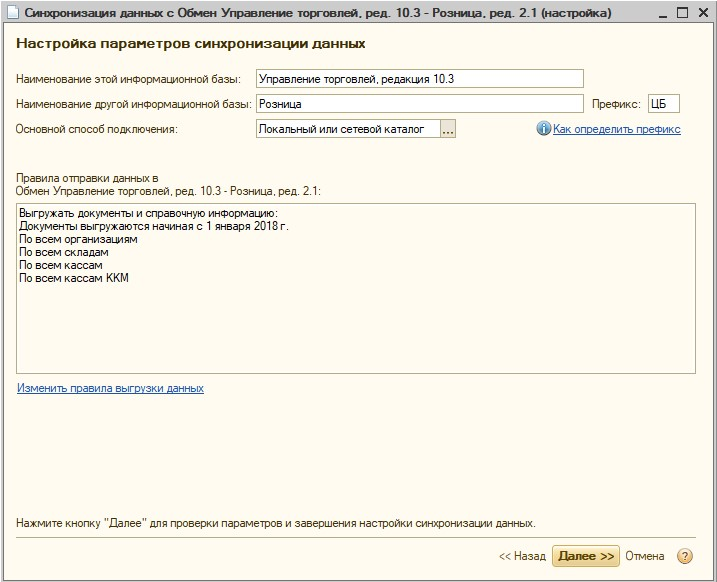
\includegraphics[width=0.8\textwidth]{8.jpg}
		\caption{Обработка загрузки данных.}
		\label{ris:8.jpg}
	\end{figure}
	
	\item На закладке «Загрузка данных» выбираем файл для загрузки.
	\item Нажимаем \keys{Загрузить данные}.
	\item Выбираем следующий файл и повторяем процесс.
\subsubsection{Порядок загрузки}	
	\item Первыми загружаем справочники. Придерживаясь порядка в дереве объектов.
	\item Вторыми загружаем регистры сведений. Придерживаясь порядка в дереве объектов.	\sidenote[-6ex][a]{Загрузка регистра себестоимости может занять достаточно продолжительное время!}
	\item Последними загружаем документы. Придерживаясь порядка в дереве объектов. \par \par
		Для корректного формирования перемещений товара в «УТ» , в «Рознице» для документов перемещающих товара должна поддерживаться следующая временная последовательность: 
	\begin{itemize}	
		\item	«Перемещение товара»
		\item	«Расходный ордер на товары»
		\item	«Приходный ордер на товары»
	\end{itemize}
	Загрузка завершена, теперь переходим к этапу проверки.\footnote{Ошибки возникающие в процессе загрузки, чаще всего связаны с необходимости корректировки правил. Так же возможны ошибки возникающие в процессе записи или проведения объекта, подобные ошибки можно проанализировать и исправить по окончанию загрузки данных}	

\end{itemize}
